\documentclass[11pt]{article}
\usepackage[margin=1in]{geometry}
\usepackage[T1]{fontenc}
\usepackage{lmodern}
\usepackage{amsmath,amssymb,amsthm}
\usepackage{graphicx,booktabs,multirow}
\usepackage[hidelinks]{hyperref}
\usepackage{microtype}
\graphicspath{{./fig/}}

\newtheorem{proposition}{Proposition}
\newcommand{\mstar}{m^{*}}

\title{A Public-Shift Softmax for Secure Inference of\\
Bounded-Attention Transformers: Cost, Failure Modes, and the Price of the Guarantee}
\author{Pol Saumell Hill\\\small Barcelona Supercomputing Center
\and Marc Casas Guix\\\small Barcelona Supercomputing Center
\and Francesc Moll\\\small Barcelona Supercomputing Center}
\date{}

\begin{document}
\maketitle

\begin{abstract}
Secure two-party transformer inference computes softmax with a secure row maximum, a log-depth tree of comparisons.
Recent systems drop it with an empirically chosen constant or clipping range, which is cheap but gives no guarantee on the
inputs' range. We observe that architectures that bound their attention logits by construction (scalar-gain query-key
normalization, attention-logit soft-capping) make a public constant shift \emph{shift-exact for every input}: the shift
cancels, and the exponential's argument lies in a known interval, so no comparison is needed. This is a guarantee about the
numerical range, not about privacy; the secure exponential and reciprocal remain approximations.
In two-party CrypTen the softmax takes a constant 37--38 rounds and, for a single softmax, communicates about $10\times$ less than
CrypTen's secure-max softmax and $13\times$ less than SHAFT's. On BERT-base, measured two-machine wall time falls by $13\%$ (128
tokens) and $24\%$ (256 tokens) against SHAFT (mean of three runs, random weights); modelled LAN/WAN gains reach $35\%/46\%$, and
the advantage vanishes at 32 tokens. A constant shift on a vanilla model, with no bound, is as fast: the speed comes from dropping the maximum, and the bound supplies the guarantee.
The guarantee has a price these costs do not include. The bound that is safe for CrypTen's 16-bit reciprocal ($g\le3$) costs
converted BERT-base $2.9$ to $14.8$ GLUE points in plaintext under one untuned recipe; most of that loss is the cap itself (SST-2 recovers to $92.3\%$ at $g\le8$ against $92.9\%$ for vanilla and $90.0\%$ at $g\le3$), while distillation and longer training recover at most $0.65$ points; a ViT trained from scratch at $g\le3$ loses $0.3\pm0.8$ points (within noise). In two-party inference of trained models on 200 SST-2 sentences and 200 QNLI pairs, the shifted softmax has a lower median logit error than the
baselines and is 5--7\% faster at about 51 tokens (QNLI) and 9.5--11\% faster at about 106 tokens (48 long QNLI pairs, faster on every pair, at a 12-point accuracy cost), but each protocol occasionally produces silent garbage logits (for the
shifted softmax, about 1 sentence in 400 on each of SST-2 and QNLI). Raising the fixed-point precision to 20 or 24 bits does not help: it makes the garbage events far more frequent. Released QK-normalized LLMs give vacuous bounds, so the bound must be designed in. On a 30-layer LLM, calibrated
constants collapsed silently under CrypTen's reciprocal.
\end{abstract}

\section{Introduction}
Secure inference for transformers is dominated by non-linear functions. In a characterization of
CrypTen-based private inference, softmax accounted for roughly half of the runtime of 12-layer
language and vision transformers, and the computation of the maximum was singled out as a key
culprit \cite{wang_ispass_2022}. The reason is structural. The stable softmax subtracts
$\max_j x_j$ so that every exponent is non-positive, but in secret-shared arithmetic a maximum is a
tree of secure comparisons, each of which is a multi-round, non-polynomial protocol. Exponentiation and
reciprocal, by contrast, admit smooth approximations.

A line of work therefore drops the maximum. NEXUS \cite{nexus_2025} uses a constant in its
softmax, THOR \cite{thor_2025} assumes inputs in a range taken from real data, and SHAFT
\cite{shaft_2025} clips inputs to an empirically tuned interval and then integrates an ODE;
ARION \cite{arion_2025} approximates the maximum by a predefined constant. These choices are
\emph{empirical}. The recent systematization of private transformer inference states the gap
directly: whether a softmax protocol can be ``non-interactive, efficient, and provably stable
without distributional assumptions remains open'' \cite{sok_2026}, and it suggests co-designing
layers to obtain tighter bounds on the softmax inputs.

\paragraph{Idea.}
Some transformer architectures already bound their attention logits to a known interval, for
stability reasons unrelated to secure computation. With query-key normalization
\cite{henry_qknorm_2020} using a scalar gain $g$, every logit is $g\cos\theta\in[-g,g]$; with
logit soft-capping \cite{gemma2_2024} every logit lies in $(-c,c)$. For such a model the shift
$\mstar=g$ (or $c$) is a public constant that is valid for \emph{all} inputs. It is exact because
it cancels, and safe because the shifted logits lie in $[-2g,0]$. No maximum, no comparison,
and for the shift itself no calibration data and no guard (a trained model's other operations still need calibrated public
scales, Section~\ref{sec:method}).

\paragraph{What we claim, and what we do not.}
A constant in place of the maximum is not new \cite{nexus_2025,thor_2025,arion_2025}; the
claims here are narrower:
\begin{enumerate}
\item the bound makes the constant valid for every input and the range of the secure exponential and reciprocal
known, and we state which conditions the fixed-point reciprocal needs; those conditions are measured for CrypTen, not
proved (Section~\ref{sec:method});
\item we measure the cost of the resulting protocol against CrypTen and SHAFT, from a single
softmax up to full BERT-base and a GPT-2-shaped decoder, including the cost of QK-norm itself
(Section~\ref{sec:cost});
\item we show, in 2-party inference of a 30-layer LLM, that calibrated constants fail silently
and increasingly under distribution shift (Section~\ref{sec:calibrated});
\item we report the price: released models do not provide a usable bound, and the bound that is
safe in fixed point costs real accuracy after conversion (Section~\ref{sec:accuracy}).
\end{enumerate}
We do not claim a free speed-up: the speed and the guarantee are bought with accuracy on
converted checkpoints, and the speed and accuracy results come from different experiments (random-weight cost
runs, plaintext fine-tuning). We tested distillation and longer fine-tuning (Section~\ref{sec:accuracy}), which recover little; we have not evaluated
QK-norm pretraining of a language model, the lever most likely to reduce that cost; the other candidate, a wider-window reciprocal in CrypTen, did not work in our tests (Section~\ref{sec:accuracy}).

\section{Background and related work}
\paragraph{Secure softmax.}
CrypTen \cite{crypten_2021} computes softmax as a secure maximum (a log-depth reduction),
an exponential by $(1+x/2^8)^{2^8}$ (eight squarings) and a Newton reciprocal. PUMA
\cite{puma_2023} and BumbleBee \cite{bumblebee_2025} also subtract the secure maximum and add a
comparison per element to clip the exponential. SHAFT \cite{shaft_2025} removes the maximum by
clipping each input to $[-4,12]$ (two ReLUs per element) and integrating an ODE for 16 steps,
for a constant 41 rounds, and states that convergence requires $\max(x)-\min(x)\le t$.
NEXUS \cite{nexus_2025} and THOR \cite{thor_2025} are homomorphic-encryption systems that use a
constant or an assumed input range; NEXUS does not say how its constant is chosen, and the SoK \cite{sok_2026}
classifies constants of this kind, in these and other HE systems, as empirically determined. Hybrid HE/MPC systems such as Iron \cite{iron_2022} and BOLT \cite{bolt_2024} use their own protocols and number formats for the softmax; our fixed-point conditions are measured for CrypTen's 16-bit reciprocal and were not evaluated there. Many systems instead replace softmax with ReLU or quadratic forms and
distill \cite{mpcformer_2023,nimbus_2024}; those are approximate and need retraining,
which differs from our setting, a shift-exact softmax on a bounded architecture.

\paragraph{Bounded attention.}
Query-key normalization \cite{henry_qknorm_2020} normalizes queries and keys to unit norm and
scales by a learnable gain.
Logit soft-capping $c\tanh(x/c)$ is used in Gemma~2 \cite{gemma2_2024}. Both were introduced
for training stability.

\section{Method}\label{sec:method}
\subsection{Exactness and a priori bounds}
For any scalar $\mstar$,
$\mathrm{softmax}(x)_i=e^{x_i-\mstar}/\sum_j e^{x_j-\mstar}$, since $\mstar$ cancels. The
maximum is needed only to keep $x_j-\mstar\le 0$. Hence any public $\mstar\ge\max_j x_j$ is exact and
safe, and the question is whether $\max_j x_j$ can be bounded \emph{before} seeing the input.

\begin{proposition}[QK-norm]
Let $\hat q_i=q_i/\|q_i\|_2$, $\hat k_j=k_j/\|k_j\|_2$ and $x_{ij}=g\,\hat q_i\!\cdot\!\hat k_j$ with a
scalar $g>0$. Then $x_{ij}\in[-g,g]$ for every input, and $\mstar=g$ gives shifted logits in $[-2g,0]$.
\end{proposition}
\begin{proof}
Cauchy--Schwarz: $|\hat q_i\!\cdot\!\hat k_j|\le\|\hat q_i\|\|\hat k_j\|=1$.
\end{proof}
\begin{proposition}[Soft-capping]
If $x=c\tanh(r/c)$ then $|x|<c$ for every raw score $r$, so $\mstar=c$ is valid before training.
\end{proposition}
With a row of $k$ visible keys the shifted exponentials lie in $[e^{-2g},1]$ and the row sum lies in
$[k\,e^{-2g},k]$, a known interval. Vanilla attention has no such bound: $|x|\le\|W_qx\|\|W_kx\|/\sqrt d$
depends on weight norms that can grow during training \cite{zhai_entropy_2023}.

\paragraph{What ``exact'' means here.} The shift is exact because it cancels; the protocol's output is not exact.
The secure exponential $(1+x/2^8)^{2^8}$ and the Newton reciprocal are approximations (the exponential's log error is
about $-14\%$ at $x{=}-8$), and the worst-case row errors we measured are $0.7$--$9.5\%$ (Section~\ref{sec:conditions}).
We say ``shift-exact'' for the first property. ``Provable'' below means a guaranteed range for the exponential's
argument; it is not a security or end-to-end accuracy guarantee.

\subsection{Threat model and what is public}
We consider semi-honest two-party computation with additive secret sharing, as in CrypTen. We make no new security
argument: the protocol composes existing CrypTen/SHAFT primitives (exponential, reciprocal, linear operations), and the
shift is data-independent. What is public must be stated, because it differs between our experiments:
the architecture (that QK-norm is used), the sequence length $N$, and an upper cap $g_{\max}$ used to choose the
reciprocal window and the public rescale $c$. The microbenchmark and the ViT experiment use a \emph{public} $g$
(the shift $m^*=g$ is a public constant); the BERT and GPT-2 cost runs use the \emph{shifted} form, where the logits are
formed as $g\cos\theta-g$ so that the shift is folded into a linear operation on shared values and the learned $g$ is not revealed.
If the model weights are private, a public per-layer $g$ leaks a trained parameter, so the shifted form is the
appropriate one; but the rescale $c$ and Eq.~\eqref{eq:cond} are then chosen from the public cap $g_{\max}$, not from the
learned $g$. The LLM experiments use public weights and secret activations; the cost runs use random encrypted weights.
The public quantities are therefore: the architecture, the sequence length $N$, the cap $g_{\max}$, the rescale $c$, and the per-layer inverse-square-root scales $c^{2}$ of Section~\ref{sec:method}. The last are calibrated on training data and are model-dependent (up to about 200 for late LayerNorms), so they reveal coarse activation statistics of the model; we did not analyse this leakage.

\subsection{Secure protocol}
Given the shared logits, the protocol is: subtract $\mstar$ (a public constant, or a shared
parameter, in which case $g$ is not revealed because subtracting a shared weight is a free linear
operation), apply the secure exponential, sum, and apply the secure reciprocal. No comparison
appears. The cost is 37--38 rounds per call, independent of the row length. QK-norm adds its own
secure operations, an inverse square root per token and head, which cost 300 extra rounds for
BERT-base; we include them in every number below.

\paragraph{Public scales for the inverse square roots.} Running a trained BERT end to end exposed a second range problem that
random-weight cost runs hide. CrypTen's Newton inverse square root, with its fixed initial guess, diverges for inputs above
roughly 75. In the trained SST-2 models the sum of squares of a query or key head vector reaches several hundred, and the
variance of a LayerNorm input row reaches about 1,500--1,800 in layers 9--10 (activation outliers); without a remedy
QK-norm's normalization failed at layer 2, and the vanilla baseline with CrypTen's own softmax failed at layer 9. We divide each
such input by a public per-layer constant $c^2$ before the inverse square root and fold $1/c$ back in
($1/\sqrt{x}=\mathrm{inv\_sqrt}(x/c^2)/c$), which adds no rounds. The constants are calibrated on 128 \emph{training}
sentences (never the evaluation ones) as $c^2=\max(1,\,3\cdot\max_{\mathrm{calib}}/25)$, giving $c^2=1$ for most layers and up
to about 200 for the late LayerNorms. We apply them identically to every variant, baselines included. The shift itself needs no
calibration, but the surrounding model does.

\subsection{Fixed-point conditions: what ``provable'' requires}\label{sec:conditions}
The bound makes the numerators representable but not automatically the reciprocal safe, and this is the
condition that matters in practice. We measured CrypTen's Newton reciprocal (16-bit fixed point,
10 iterations, 2-party, 64 repetitions per point) and found it within 1\% only for
$\ln s\in[-6.5,+3.0]$; the error is 4.3\% at $+4.0$, 30\% at $+5.0$, and the output is garbage for
$\ln s\ge 5.5$ (a row sum $\ge 256$); at the low end it is 2.6\% at $-8$ and 36\% at $-9$
(under-converged). A public rescale $1/s=(1/(s/c))/c$ costs two public multiplications and no
communication, and shifts the window. With $c=\max(1,N/64)$ and $k_{\min}$ the fewest visible keys in
any row, we find the lower end is the binding constraint:
\begin{equation}
2g+\ln c\;\le\;6.75+\ln k_{\min}.\label{eq:cond}
\end{equation}
At $k_{\min}=1$ (a causal decoder) and $N\le128$ this gives $g\le 3$; $g=5.5$ is not safe, because a row
whose only visible key sits at $-2g$ has $\ln s=-11$, far outside the window. We stress that
\eqref{eq:cond} is derived from measurements of this specific reciprocal, not proved, and holds for
the tested range ($N\le512$, six row kinds, $g\in\{3,5.5\}$).

\section{Cost evaluation}\label{sec:cost}
\paragraph{Setup.}
All protocols run in 2-party CrypTen using SHAFT's fork (torch 2.0.1), 16-bit fixed point, on
MareNostrum~5 general-purpose nodes (Xeon 8480+). Cost is weight-independent, so BERT/GPT-2
costs use random encrypted weights; rounds and bytes are exact and deterministic. Three softmaxes:
CrypTen's secure max; SHAFT's clip + ODE ($t=16$); and ours (QK-norm + shifted softmax).
Network time uses SHAFT's model (compute $+\,8\cdot$bytes/bandwidth $+$ rounds$\cdot$latency; LAN
3\,Gbps/4\,ms, WAN 400\,Mbps/40\,ms); we also measure wall-clock on two machines.

\subsection{Single softmax}
Per 16-row batch, $n=1024$ (inputs in $[-g,g]$): CrypTen 137 rounds, 22.8\,MB, 185\,ms;
SHAFT 41 rounds, 32.0\,MB, 129\,ms; ours 37 rounds, 2.37\,MB, 41\,ms. Ours is
$9.6\times$ and $13.5\times$ smaller in communication and $4.5\times$/$3.1\times$ faster.
CrypTen's secure-max softmax also breaks at long rows: at $n=1024$, flat rows give errors of
$10^{7}$--$4\times10^{9}$ at both precisions, while ours stays at $10^{-4}$. Removing the maximum
removes that failure mode too. SHAFT's ODE is about $11\times$ less accurate than ours on peaked
rows (max error 0.17 vs 0.015).

\subsection{BERT-base and a causal decoder}
Table~\ref{tab:bert} gives BERT-base (12 layers, hidden 768) encoder cost. Softmax shrinks from
38--55\% of the bytes to a few percent (Figure~\ref{fig:bytes}); GELU becomes the largest cost.
QK-norm costs 300 extra rounds (total 1704 vs SHAFT's 1440, $+18\%$) but only 0.1--0.2\,GB.

\begin{table}[t]\centering\small
\caption{BERT-base encoder, 16-bit, 2 parties, random weights (N = tokens). Wall time is the mean of three runs, measured on two
machines; LAN/WAN are modelled.}\label{tab:bert}
\begin{tabular}{@{}rlrrrrr@{}}\toprule
N & Softmax & Rounds & GB & Wall (s) & LAN (s) & WAN (s)\\\midrule
\multirow{3}{*}{32} & CrypTen max & 2208 & 2.78 & -- & 32.8 & 160.5\\
 & SHAFT & 1440 & 2.85 & -- & 29.5 & 130.7\\
 & Ours & 1704 & 2.61 & -- & 29.5 & 136.1\\\midrule
\multirow{3}{*}{128} & CrypTen max & 2340 & 9.70 & 54.9 & 90.0 & 342.5\\
 & SHAFT & 1440 & 10.80 & 55.3 & 90.3 & 329.3\\
 & Ours & 1704 & 6.68 & \textbf{47.9} & \textbf{72.8} & \textbf{249.8}\\\midrule
\multirow{3}{*}{256} & CrypTen max & 2460 & 24.16 & 116.8 & 192.1 & 699.5\\
 & SHAFT & 1440 & 29.52 & 124.0 & 209.5 & 773.1\\
 & Ours & 1704 & 12.83 & \textbf{94.1} & \textbf{135.6} & \textbf{419.3}\\\bottomrule
\end{tabular}

\smallskip
\begin{minipage}{.92\linewidth}\footnotesize
\emph{Notes.} Wall: two Xeon 8480+ nodes (23\,Gbps link, 56 threads per party), $N{=}128$ and 256 only. Rounds, GB, LAN and
WAN come from the single-node run; LAN/WAN apply SHAFT's time model to that run's compute time, so they mix two runs with the
Wall column (their totals differ by up to about 1\,s). The Wall column is the mean of three runs on the same two nodes (standard deviation at most 0.3\,s); rounds and bytes are deterministic; LAN and WAN come from one run. CrypTen and SHAFT run
unmodified, without the public rescale given to ours, so the CrypTen cells at $N{=}256$ are not like-for-like.
\end{minipage}
\end{table}

\begin{figure}[t]\centering
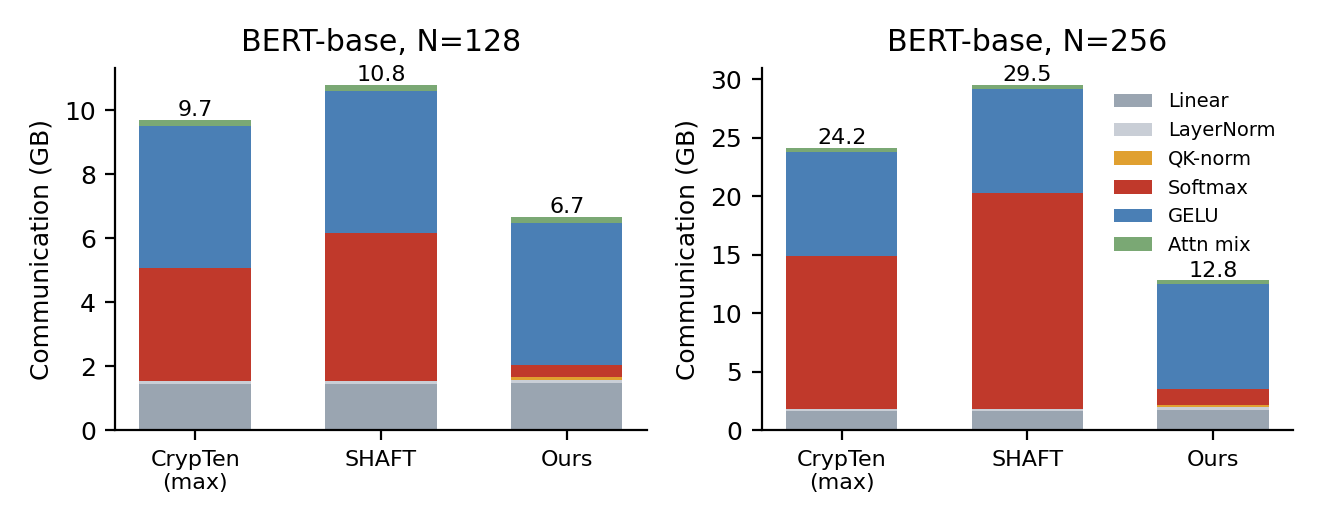
\includegraphics[width=.9\linewidth]{mpc_bytes.png}
\caption{Communication by component, BERT-base, two-node run. Softmax dominates the baselines and
is small in ours; QK-norm adds a small slice.}\label{fig:bytes}
\end{figure}

Against SHAFT, the measured two-machine wall time falls by 13.4\% at $N{=}128$ and 24.1\% at
$N{=}256$; against CrypTen by 12.9\% and 19.5\% (means of three runs). End-to-end bytes fall by 31\% and 38\% at 128 tokens and by 47\% and 57\%
at 256 tokens against CrypTen and SHAFT (the $10\times$ and $13\times$ figures belong to the single softmax).
The wall-time gap against SHAFT is mostly SHAFT's 16-step ODE: at $N{=}128$ the softmax takes 9.5\,s for SHAFT,
8.9\,s for CrypTen's secure max and 1.3\,s for ours, so against CrypTen the gain is the smaller one. The three runs agree to within 0.3\,s (standard deviation), and the two-node and single-node totals agree within 1.5\%. The modelled LAN/WAN reductions against SHAFT are
19.4\%/24.1\% at 128 and 35.3\%/45.8\% at 256. With the embedding, pooler and classifier included
($N{=}128$) they are 17.4\%/22.7\%. A GPT-2-shaped causal decoder (prefill, blocks only, public
mask sent to $-30$) behaves the same: $-19.3\%$ (LAN) and $-24.0\%$ (WAN) at 128, and $-35.0\%$ and $-45.7\%$ at 256.
Under QK-norm the shifted logits lie in $[-2g,0]$, so the $-30$ mask rounds to exactly zero.

\paragraph{Caveats on these numbers.}
\begin{enumerate}\setlength{\itemsep}{1pt}
\item At $N{=}32$ the extra QK-norm rounds cancel the byte savings (LAN $+0.2\%$, WAN $+4.2\%$ vs SHAFT): there is no gain
for short inputs.
\item The two-node link is fast (23\,Gbps, 0.16\,ms) and communication is only 3--5\% of wall time there, so the measured
advantage is a compute advantage. The LAN and WAN rows remain \emph{modelled}; the model over-predicts measured
communication by $1.35$--$1.65\times$ on this link (with the byte term scaled by $0.6$ the reductions at 128 tokens are
$16.3\%/19.0\%$, same ranking). A real WAN was not run.
\item Raising the Newton iterations to 20 for a wider reciprocal window adds 240 rounds and moves the 128-token gain to
$-18.1\%$ (LAN) and $-21.2\%$ (WAN).
\item The headline comparison gives the baselines no public rescale and a clip range not tuned to bounded logits.
Table~\ref{tab:fair} (below) adds fairness controls: CrypTen with the same rescale, SHAFT with a narrowed clip, and a constant shift on a vanilla model
without QK-norm.
\item Table~\ref{tab:bert} is measured with random weights. Rounds and bytes do not depend on the values, but the fixed-point
behaviour does, and trained weights needed the public scales of Section~\ref{sec:method}. Section~\ref{sec:accuracy} reports a
trained model at about 26 tokens, where there is no speed-up.
\item Our SHAFT total at $N{=}128$ with the embedding (11.25\,GB) differs from SHAFT's paper (10.46\,GB), plausibly because of
our one-hot embedding and a CrypTen-level reimplementation of the encoder (SHAFT's ONNX path did not import the QK-norm graph).
\item These costs do not depend on $g$. The accuracy of models that satisfy Eq.~\eqref{eq:cond} is in
Section~\ref{sec:accuracy}.
\end{enumerate}

\paragraph{Fairness controls.} Table~\ref{tab:fair} reruns BERT-base on a single node with three controls (random weights; cost
only for the last two). \emph{CrypTen with our public rescale} has identical rounds and bytes (a public multiplication costs nothing).
\emph{SHAFT with the clip narrowed to $[-6,0]$ and 8 ODE steps} (what a bounded model would allow; its accuracy was not
validated) saves 192 rounds and about 1.2--4.8\,GB, and ours remains $10\%$ ($N{=}128$) and $19\%$ ($N{=}256$) faster in wall
time and uses about $48\%$ fewer bytes at 256 tokens. \emph{A constant shift on a vanilla model without QK-norm} is as fast as ours
and $0.7$--$2.3\%$ faster (it lacks the 300 QK-norm rounds), but it carries no bound. So the speed comes from dropping the
secure maximum, which prior systems already do; what the architecture adds is the guarantee on the shift, at the price of
$0.7$--$2.3\%$ of the time and of the accuracy losses of Section~\ref{sec:accuracy}.

\begin{table}[t]\centering\footnotesize\setlength{\tabcolsep}{4pt}
\caption{Fairness controls, BERT-base encoder, single node, random weights, one run, 16-bit. Wall = measured seconds on one node
(loopback), so values differ slightly from Table~\ref{tab:bert}. The two starred rows are cost only.}\label{tab:fair}
\begin{tabular}{@{}lrrrrrr@{}}\toprule
 & \multicolumn{3}{c}{$N=128$} & \multicolumn{3}{c}{$N=256$}\\\cmidrule(lr){2-4}\cmidrule(lr){5-7}
Softmax & Rounds & GB & Wall (s) & Rounds & GB & Wall (s)\\\midrule
CrypTen max & 2340 & 9.70 & 56.4 & 2460 & 24.16 & 118.7\\
CrypTen max + our rescale & 2340 & 9.70 & 55.9 & 2460 & 24.16 & 118.8\\
SHAFT (clip $[-4,12]$, 16 steps) & 1440 & 10.80 & 56.6 & 1440 & 29.52 & 125.4\\
SHAFT narrowed ($[-6,0]$, 8 steps)* & 1248 & 9.59 & 54.1 & 1248 & 24.69 & 116.5\\
Constant shift, no QK-norm* & 1392 & 6.54 & 47.5 & 1392 & 12.48 & 93.9\\
Ours (QK-norm + shifted) & 1704 & 6.68 & 48.6 & 1704 & 12.83 & 94.6\\\bottomrule
\end{tabular}
\end{table}

\subsection{Worst-case rows}
We ran 16 rows each of six kinds (all logits at $-2g$, all at 0, one at 0, one visible key at
$-2g$ as in a causal first token, uniform over $[-2g,0]$, and trained-like cosines) for
$g\in\{3,5.5\}$, $N\in\{32,\dots,512\}$. With $g\le3$ and $c=\max(1,N/64)$ no row produced garbage
up to $N{=}512$; the worst row-sum error is $\le0.7\%$ to 128 tokens and 1.45\% at 256, versus
0.1--2.4\% for CrypTen's own softmax, which produces garbage on uniform rows at $N\ge256$ because its
row sums reach $N$. At 512 our worst case is 9.5\% (the one-key causal row loses resolution when
divided by $c=8$). With $g=5.5$, the one-key row (ln\,$s=-11$, outside the window; 87\% error in the fine sweep) produced
garbage at every $N$ tested, as Eq.~\eqref{eq:cond} predicts. Calls take 38 rounds against 106--137.

\section{Calibrated constants on an unbounded LLM under CrypTen's reciprocal}\label{sec:calibrated}
Since a calibrated constant needs no architecture change, the natural alternative is to profile one.
We ran SmolLM2-135M (all 30 decoder layers, weights public, activations secret, embedding lookup
and LM head in the clear) in 2-party CrypTen at 16 bits on 64-token windows. The plaintext
reimplementation matches Hugging Face (KL $5$--$9\times10^{-6}$, identical perplexity). Constants were
calibrated on 128 Wikitext windows ($+1$ nat) at layer, head, and head$\times$position granularity.

\paragraph{Plaintext statistics.} 43--46\% of rows underflow at 16 bits with a per-layer constant,
and 4--5\% with a per-head constant, even on the calibration domain. At the finest granularity the
share of windows containing a row the reciprocal cannot handle is 3.1\% on held-out Wikitext, 0--1.6\%
on Spanish/Catalan, 6.2\% on math, 17.2\% on chat and 31--39\% on code, with the per-row excess over
the constant reaching $+12.5$ nats on code ($+7.7$ on Wikitext). Separately, a layer-wide constant
profiled on Wikitext is exceeded by 9.2--9.4 nats on code for both SmolLM2 and TinyLlama and by
4--5.6 nats on Catalan and Spanish (plaintext attention); FP32 absorbs this, 16-bit secure arithmetic
does not.

\paragraph{Secure runs.} With CrypTen's secure maximum, 9/9 windows are fine (top-1 agreement
0.98--1.00 with plaintext, perplexity within about 1--2\%). With a calibrated constant every
granularity collapses (Table~\ref{tab:llm}; LAN/WAN are modelled from per-window times aggregated as in our run logs, and recomputing from the raw CSV mean gives values
1--2\,s higher): per-layer and per-head constants fail on all windows;
the finest per-row constant fails on 8 of 9, including in-distribution windows; 20 Newton iterations
make it worse (9/9 collapsed). The mechanism is that a handful of rows per layer (0.2--0.3\% underflow, 2--3\%
short of the reciprocal's range) produce a reciprocal that overflows the 2-party truncation, and one such
row per layer is enough across 30 layers. With a public floor $e^{-6}$ on the row sum (job v3, 32 windows, four
domains), outcomes are \emph{garbage} on 3/8 held-out Wikitext windows and 6/8 HumanEval windows. The
failure rate rises with how far the data exceed the constant (Figure~\ref{fig:excess}): 27\%
(excess $<3$ nats), 46\% (3--6), 88\% ($\ge6$). Outputs stay finite, so a non-finite guard would not fire.

\begin{table}[t]\centering\small
\caption{Secure SmolLM2-135M, 16-bit, 9 windows (v2). Collapsed = non-finite, top-1 $<0.5$ or perplexity $\times2$.}\label{tab:llm}
\begin{tabular}{@{}lccc@{}}\toprule
Softmax & Collapsed W/code/Catalan & Mean top-1 (W/code/ca) & LAN / WAN (s)\\\midrule
CrypTen secure max & 0/3, 0/3, 0/3 & .98 / .99 / .98 & 55.5 / 337.3\\
Constant per layer & 3/3, 3/3, 3/3 & .02 / .00 / .01 & 38.0 / 212.0\\
Constant per head & 3/3, 3/3, 3/3 & .01 / .02 / .04 & 38.0 / 212.0\\
Constant per head$\times$position & 3/3, 3/3, 2/3 & .04 / .27 / .53 & 38.0 / 212.0\\\bottomrule
\end{tabular}
\end{table}

\begin{figure}[t]\centering
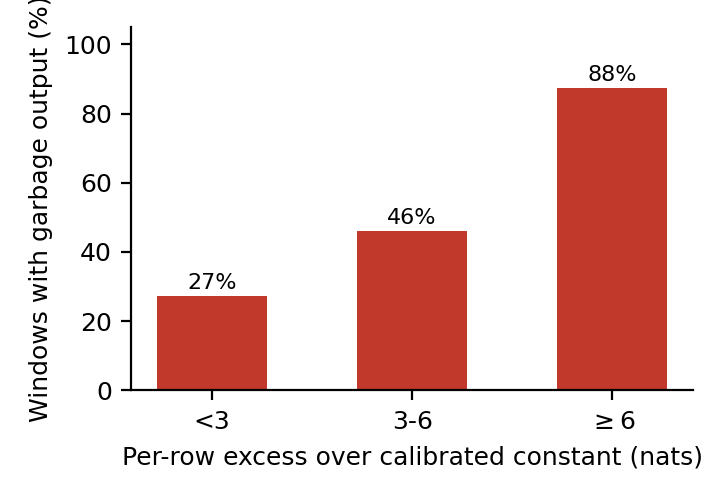
\includegraphics[width=.5\linewidth]{mpc_excess.png}
\caption{Fraction of windows with garbage output vs per-row excess over the calibrated constant
(floor $e^{-6}$, 32 windows). Few windows per bin (8--13); read the trend, not individual rates.}\label{fig:excess}
\end{figure}

Three scope notes. (1)~This is a statement about CrypTen's 16-bit reciprocal: the collapse is a cliff caused by a few rows whose sum leaves the
reciprocal's working range, and a range-extended reciprocal, more precision, or a clamp of the row sum might
rescue a calibrated constant; we did not try these, so the section shows that calibrated constants are fragile under this
reciprocal, not that they cannot work. (2)~We ran 8--9 windows per domain and one model, with bins of 8--13 windows built from four domains and no
confidence intervals, so read the trend, not individual rates. (3)~We could not separate this failure from model type: a test of input-level distribution shift on pre-LN ViTs
never pushed attention past a clean-calibrated constant (0 of 266,240 rows), so we make the claim
only for language models.

\section{The price of the guarantee}\label{sec:accuracy}
\paragraph{Released models give no bound.} Computed from the released weights, the logit bounds of per-dimension QK-norm models are
enormous: 184--12,897 nats for Qwen3-0.6B,
183--5,361 for Qwen3-1.7B, and 995--4,267 for OLMo-2-1B; Gemma~2's soft-cap $c=50$ gives a 100-nat width.
None fits a 16-bit range ($\approx 11$ nats). A usable bound must be designed in: a scalar gain
with a small cap, trained or fine-tuned in.

\paragraph{Vision.} A CIFAR-10 ViT trained from scratch with scalar QK-norm reaches 81.74\% against
81.24\% vanilla, logits in $[-4.29,4.38]\subset[-4.48,4.48]$, so $\mstar=g$ is exact without profiling.
In 2-party inference of that model (200 images, one run, public $g$) the shifted softmax gives 99.0\% agreement with
plaintext (CrypTen max 98.5\%, SHAFT 99.0\%) with the least communication of five variants (94.3 vs 177.8--215.9\,MB per image).
At 65 tokens the extra QK-norm rounds cancel the byte savings (WAN $+3\%$ vs vanilla+SHAFT).

\paragraph{Converted BERT-base.} We convert BERT-base to scalar-gain QK-norm and fine-tune it for
3 epochs (lr $2\!\times\!10^{-5}$, gains at $10^{-3}$, one recipe for all tasks, not tuned). Table~\ref{tab:glue} shows
the result: the bound that Eq.~\eqref{eq:cond} requires ($g\le3$) costs $2.9$--$14.8$ points under this single untuned recipe, which is mostly the cost of the cap itself (the gains sit at the cap; sweeps of the cap, of the recipe and a from-scratch ViT control follow below); even $g\le5.5$, which is not
provable for single-key rows, costs $1.0$--$4.8$.
SST-2 is the mildest task. The gains sit at the cap on every task, so the bound binds. The mechanism is that $g$ caps
attention sharpness: the largest weight a single key can receive among $N$ is $e^{2g}/(e^{2g}+N-1)$, i.e.\ 0.76 at
$g=3$, $N=128$ (0.998 at $g=5.5$), which hurts tasks needing token-level attention (CoLA, RTE, MRPC); the cap sweep below supports this.

\begin{table}[t]\centering\small
\caption{GLUE dev, BERT-base converted from the vanilla checkpoint (mean $\pm$ sd over seeds: 5 for RTE, MRPC and CoLA; 3 for QNLI, MNLI and SST-2).
Metric: accuracy; MRPC F1; CoLA Matthews.}\label{tab:glue}
\begin{tabular}{@{}lrrr@{}}\toprule
Task & Vanilla & $g\le5.5$ & $g\le3.0$ (fixed-point safe)\\\midrule
SST-2 & 92.89$\pm$0.30 & 91.93$\pm$0.29 & 89.95$\pm$0.63\\
QNLI & 91.48$\pm$0.20 & 89.33$\pm$1.48 & 86.36$\pm$0.90\\
MNLI-m & 84.38$\pm$0.17 & 83.16$\pm$0.30 & 80.58$\pm$0.12\\
MRPC (F1) & 88.57$\pm$1.25 & 85.10$\pm$0.80 & 83.14$\pm$1.32\\
RTE & 62.31$\pm$0.94 & 57.47$\pm$2.47 & 55.02$\pm$2.48\\
CoLA (MCC) & 57.28$\pm$1.43 & 54.42$\pm$1.02 & 42.53$\pm$3.22\\\bottomrule
\end{tabular}
\end{table}

\begin{figure}[t]\centering
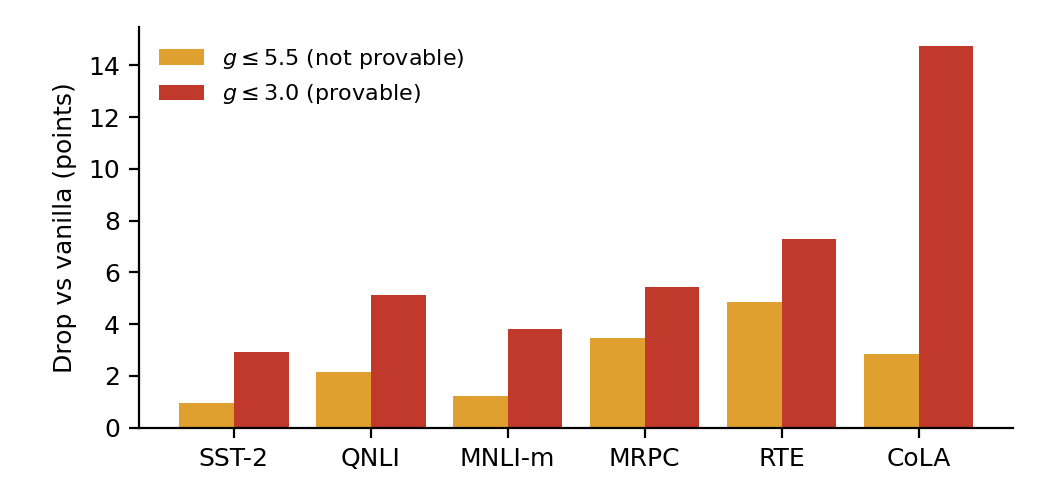
\includegraphics[width=.62\linewidth]{mpc_glue.png}
\caption{Accuracy drop of QK-norm-converted BERT-base against vanilla.}\label{fig:glue}
\end{figure}

\paragraph{How much of the cost is the cap, and how much the recipe?} We ran three controls. \emph{Accuracy against the cap}
(Table~\ref{tab:gsweep}; same recipe, 3 seeds on SST-2, 1 seed on QNLI for the new points): accuracy rises steadily as the cap is relaxed. On
SST-2 it goes from $89.95$ at $g\le3$ to $91.09$ at $g\le4$, $91.93$ at $5.5$ and $92.28$ at $8$, against $92.89$ for vanilla; it is flat beyond
$8$ ($92.24$ at $12$). On QNLI, $g\le8$ reaches $91.45$ (one seed) against $91.48$ for vanilla. So most of the conversion loss is the cap
itself, and a cap near 8 costs under a point here; but only $g\le3$ is safe for CrypTen's 16-bit reciprocal (Eq.~\eqref{eq:cond}).
\emph{Recipe variants} (Table~\ref{tab:var}, SST-2, $g\le3$, 3 seeds each): distilling from the vanilla fine-tuned model, a higher learning
rate, or 10 epochs alone leave accuracy within noise of the baseline recipe ($89.83$--$90.06$ against $89.95$); distillation with 10 epochs gives
$90.60\pm0.41$, so recipe changes recover at most $0.65$ points (about one standard deviation with three seeds). The recipe controls and the
sweep were scored on the dev set that Table~\ref{tab:glue} also uses, so they are sensitivity analyses, not tuned results.
\emph{ViT trained from scratch with $g\le3$} (CIFAR-10, 100 epochs, 3 seeds): vanilla $81.32\pm0.19$ against QK-norm
$81.01\pm0.74$ (QK-norm seeds $81.50$, $80.15$, $81.39$; vanilla $81.24$, $81.18$, $81.53$). The learned gain is $2.84$, the logits lie in
$[-2.79,2.79]$, and the shift error is about $10^{-7}$. The $0.3$-point gap is within seed noise, which with three seeds does not exclude a loss of
one to two points. Taken together: for a pre-trained BERT converted to scalar-gain QK-norm, the cap is the main driver of the loss and the training
recipe is not; a model trained with a $g\le3$ cap from the start (a small ViT) loses little, so the cap hurts most when a pre-trained model's
sharp attention is forced under it. This is thin evidence (one small ViT, two language tasks, no language model pre-trained with the bound).

\begin{table}[t]\centering\small
\caption{BERT-base accuracy (dev, \%) against the gain cap, same recipe (3 epochs, lr $2\!\times\!10^{-5}$). Mean $\pm$ sd over 3 seeds
unless marked; $^\dagger$ one seed; -- not run. Only $g\le3$ is fixed-point safe for CrypTen's 16-bit reciprocal.}\label{tab:gsweep}
\begin{tabular}{@{}lcc@{}}\toprule
Cap $g_{\max}$ & SST-2 & QNLI\\\midrule
3 (safe) & 89.95$\pm$0.63 & 86.36$\pm$0.90\\
4 & 91.09$\pm$0.13 & --\\
5.5 & 91.93$\pm$0.29 & 89.33$\pm$1.48\\
8 & 92.28$\pm$0.18 & 91.45$^\dagger$\\
12 & 92.24$\pm$0.46 & --\\
Vanilla & 92.89$\pm$0.30 & 91.48$\pm$0.20\\\bottomrule
\end{tabular}
\end{table}

\begin{table}[t]\centering\small
\caption{BERT-base SST-2 with $g\le3$: recipe variants (dev accuracy \%, 3 seeds). KD = distillation from the vanilla fine-tuned
model.}\label{tab:var}
\begin{tabular}{@{}lccc@{}}\toprule
Recipe & Epochs & lr & Mean $\pm$ sd\\\midrule
Baseline & 3 & $2\!\times\!10^{-5}$ & 89.95$\pm$0.63\\
KD & 3 & $2\!\times\!10^{-5}$ & 89.83$\pm$0.47\\
Higher lr & 3 & $5\!\times\!10^{-5}$ & 90.06$\pm$0.52\\
Longer & 10 & $2\!\times\!10^{-5}$ & 90.02$\pm$0.69\\
KD, longer & 10 & $2\!\times\!10^{-5}$ & 90.60$\pm$0.41\\\bottomrule
\end{tabular}
\end{table}

\paragraph{Secure inference of the converted BERT.} We ran the SST-2 models end to end in two-party CrypTen (16-bit): the
$g\le3$ QK-norm model with the shifted softmax, and the vanilla model with CrypTen's secure max and with SHAFT's ODE, on the same
200 validation sentences (a seeded random subset; mean 25.9 tokens, no padding, so every row has all keys visible). Weights are
secret-shared by party~0; the embedding output of each sentence is computed by the client (party~1) and encrypted; the encoder,
pooler and classifier are secure. The $g\le3$ model is the seed-0 model from Table~\ref{tab:glue} (90.25\% on the full dev set).
Table~\ref{tab:sec} gives the results. The converted model's secure predictions agree with its plaintext predictions on 200 of
200 sentences, and the secure accuracy equals its plaintext accuracy (91.0\%), 1.0 point below the secure vanilla model (92.0\%),
as in plaintext on this subset. \textbf{This agreement overstates the numerical quality:} on one sentence (41 tokens) the secure
logits were garbage ($-8\times10^{8}$ and $-2\times10^{8}$ against plaintext $-3.0$ and $+3.1$), and the class was right only
because the garbage values happened to be ordered the right way round. The output was finite, so a non-finite guard would not
fire. CrypTen's secure max failed the same way once (26 tokens), and there it flipped the prediction; SHAFT's ODE produced no
garbage logits (maximum error 0.68) but disagreed with plaintext once. Rerunning each of the two failing sentences alone, three times with fresh randomness, gave no failure (6 of 6 runs with maximum error
0.02--0.05), so the failures are not determined by the input; they depend on the shares or the run state. A full second pass of the $g\le3$ model over the same 200 sentences with fresh randomness had no sentence with error above 1, including
the one that failed before, and its logits differ from the first pass by a median of $0.002$ (maximum $0.019$). The failure is therefore a rare event driven by the
randomness of the shares, about 1 in 400 sentence runs for this model on SST-2. We tested one candidate cause, CrypTen's probabilistic truncation, whose failure probability grows with the magnitude of the fixed-point values: on 40 sentences, raising the precision from 16 to 20 bits made 16 of 40 sentences garbage for the shifted softmax and 18 of 40 for the secure max (against about 1 in 400 at 16 bits), and at 24 bits every sentence was wrong for both. The direction fits the hypothesis, the effect is the same for both protocols, and it rules out ``more bits'' as a remedy in CrypTen; we did not isolate truncation from other overflows. With such a low rate at 16 bits we cannot rank the softmaxes. At this sequence length the converted model is not meaningfully faster
($15.5$\,s against $16.5$\,s for the secure max and $15.7$\,s for the ODE per sentence) and uses more rounds than the ODE,
consistent with the absence of a gain at 32 tokens in Table~\ref{tab:bert}.

\begin{table}[t]\centering\footnotesize\setlength{\tabcolsep}{4pt}
\caption{Secure two-party inference of fine-tuned BERT-base on 200 SST-2 validation sentences (mean 25.9 tokens), 16-bit, one
seed; same public scales for every row. Plain/Secure = accuracy (\%); err = max$|$secure $-$ plaintext logit$|$ per sentence; garb. = sentences with err $>1$.
Costs are means per sentence.}\label{tab:sec}
\begin{tabular}{@{}lrrrrrrr@{}}\toprule
Model, softmax & Plain & Secure & Agree & Med.\ err & Garb. & Rounds / GB & s\\\midrule
QK-norm $g\le3$, shifted (ours) & 91.0 & 91.0 & 200/200 & 0.023 & 1 & 1790 / 2.40 & 15.5\\
Vanilla, CrypTen max & 92.5 & 92.0 & 199/200 & 0.033 & 1 & 2211 / 2.53 & 16.5\\
Vanilla, SHAFT ODE & 92.5 & 92.0 & 199/200 & 0.036 & 0 & 1490 / 2.57 & 15.7\\\bottomrule
\end{tabular}
\end{table}

\paragraph{Longer inputs: QNLI.} SST-2 sentences are short, so we repeated the experiment on QNLI (question and sentence pairs; 200
seeded validation pairs, mean 51.3 tokens, up to 128), with the same recipe and public scales; the main $g\le3$ model is the seed-0
model (87.0\% on the full dev set, against 91.3\% for vanilla); a second seed is reported below. Table~\ref{tab:qnli} gives the results. The shifted softmax is faster
than both baselines on every sentence pair compared: by $7.4\%$ against CrypTen's secure max and $5.5\%$ against SHAFT's ODE
(per-sentence paired differences; 95\% intervals $\pm0.2$ and $\pm0.3$ points, which reflect sentence-to-sentence variation only, since the
three runs were separate jobs on different nodes of the same type), with $11\%$ and $15\%$ fewer bytes. The median logit error is five
times smaller ($0.074$ against $0.40$ and $0.45$), and 1 sentence has an error above 1 against 8 and 19. The catastrophic failure
recurs: one sentence (72 tokens) produced garbage logits ($\sim\!10^{5}$ in error) under the shifted softmax, and one under SHAFT's ODE
(a different sentence). Rerun alone three times each, neither reproduced (errors $0.08$ and $0.23$), as on SST-2, so 12 of 12 isolated
reruns of the four failing sentences were clean; CrypTen's max produced none here, although it had one in the SST-2 run. Secure and plaintext predictions
agree on 199, 198 and 196 of 200 sentences; the flipped predictions of the $g\le3$ model fall on a sentence whose plaintext logits differ by
$0.014$, so they are near-ties. The secure accuracy of the converted model stays 4 points below the secure vanilla model, as in plaintext.
A second QNLI seed of the converted model (full dev accuracy 86.75\%, against 87.00\%) behaves similarly and has no catastrophic failure: secure
accuracy 88.5\% (plaintext 88.0\%) on the same 200 pairs, agreement 199/200, median error $0.035$, no sentence with error above 1, the same
1790 rounds and 3.45\,GB, and $6.6\%$ and $4.7\%$ faster than CrypTen's max and SHAFT's ODE (it is faster than the ODE on 194 of 200 pairs). The
catastrophic failure therefore occurred for one of the two QNLI models (1 sentence in 400 for the shifted softmax on QNLI); the two seeds differ in
their weights, so these are not two draws of the same experiment. The speed gain at 51 tokens is much smaller than the 13--24\% measured at 128--256 tokens with random weights, as the cost model predicts.

\begin{table}[t]\centering\footnotesize\setlength{\tabcolsep}{4pt}
\caption{Secure two-party inference of fine-tuned BERT-base on 200 QNLI validation pairs (mean 51.3 tokens), 16-bit, seed-0 converted
model; same public scales for every row. Err $>1$ / $>10$ = sentences whose maximum logit error exceeds 1 / 10. Costs are means per sentence.}\label{tab:qnli}
\begin{tabular}{@{}lrrrrrrrr@{}}\toprule
Model, softmax & Plain & Secure & Agree & Med.\ err & Err$>$1 & Err$>$10 & Rounds / GB & s\\\midrule
QK-norm $g\le3$, shifted (ours) & 86.5 & 87.0 & 199/200 & 0.074 & 1 & 1 & 1790 / 3.45 & 23.9\\
Vanilla, CrypTen max & 91.0 & 91.0 & 198/200 & 0.395 & 8 & 0 & 2305 / 3.95 & 25.9\\
Vanilla, SHAFT ODE & 91.0 & 91.0 & 196/200 & 0.448 & 19 & 1 & 1490 / 4.14 & 25.5\\\bottomrule
\end{tabular}
\end{table}

\paragraph{Long inputs.} The speed and accuracy results above are at about 51 tokens, where the gain is 5--7\%. To put speed and accuracy at one operating point at a length where the gain is larger, we evaluated the 48 QNLI dev pairs with at least 90 tokens (mean 106) with the same three models (Table~\ref{tab:long}; one run per pair). The shifted softmax is 9.5\% faster than the secure max and 11.1\% faster than the ODE, and faster on all 48 pairs. The cost of the cap is also larger on these inputs: 79.2\% plaintext accuracy against 91.7\% for vanilla (secure 81.2\%, a 2-pair difference). Garbage logits again occur for every protocol (1, 4 and 5 pairs); the counts are too small to rank them.

\begin{table}[t]\centering\small
\caption{Long QNLI pairs ($\ge90$ tokens, $n=48$, mean 106 tokens), 2-party CrypTen on two MN5 nodes. Columns as in Table~\ref{tab:qnli}.}\label{tab:long}
\begin{tabular}{@{}lrrrrrrr@{}}\toprule
Model, softmax & Plain & Secure & Agree & Med.\ err & Err$>$1 & Rounds / GB & s\\\midrule
QK-norm $g\le3$, shifted (ours) & 79.2 & 81.2 & 45/48 & 0.174 & 1 & 1790 / 5.79 & 42.4\\
Vanilla, CrypTen max & 91.7 & 91.7 & 46/48 & 0.463 & 4 & 2390 / 7.79 & 46.9\\
Vanilla, SHAFT ODE & 91.7 & 91.7 & 46/48 & 0.499 & 5 & 1490 / 8.56 & 47.8\\\bottomrule
\end{tabular}
\end{table}

\section{Discussion and limitations}
\paragraph{Where this leaves the trade-off.} The speed result (Section~\ref{sec:cost}) and the
accuracy result (Section~\ref{sec:accuracy}) are measured on the same protocol but not on the same
operating point as a deployment would choose: the cost does not depend on $g$, while the guarantee does.
The honest summary is that, for a model that is \emph{already} bounded (or can be retrained so), a
shift-exact, comparison-free softmax is a clear communication saving; for a converted model it is a speed/accuracy trade of
several points on harder tasks.
A wider reciprocal window, the lever we expected to relax the cap, was tested in CrypTen and failed: 20 Newton iterations at 16 bits and 10 iterations at 24 bits both left the shifted softmax producing garbage rows at $g=5.5$ and $8$ (the secure max did not at 128 tokens or fewer), so the cap is set by CrypTen's reciprocal and truncation together, not by the window alone. Two levers could change the trade-off and were not tested: QK-norm pretraining (distillation and longer fine-tuning were tested and recover at most 0.65 points on SST-2), and a
softmax with a constant in the denominator (``softmax-one'') or a public floor on the row sum. The last changes the function (it is no longer
the exact softmax) unless it is a floor applied only for numerical safety, and a floor of $e^{-6}$ did not rescue
calibrated constants on the LLM.

\paragraph{Limitations.}
\begin{enumerate}\setlength{\itemsep}{1pt}
\item Fixed-point conditions come from measuring one reciprocal implementation (CrypTen's), not from a proof.
\item LAN/WAN numbers use SHAFT's time model; wall-clock is on a fast link.
\item The large cost tables use random weights. Secure accuracy of the converted BERT was measured on two tasks (SST-2, QNLI),
200 sentences each (about 26 and 51 tokens) plus 48 long QNLI pairs (about 106 tokens), one seed for most runs, and not on the other GLUE tasks.
\item Decoder results are prefill cost only and no QK-norm decoder was trained. Decode-phase cost with a KV cache, where a
secure maximum over one row costs about $\log_2 t$ rounds, is not measured, and the advantage there is likely smaller.
\item The calibrated-constant failure is for an unbounded LLM at 16 bits in CrypTen, from few windows.
\item We evaluate semi-honest 2-party computation in one framework; the argument that the shift can be public or shared
composes existing protocols and is not a new security proof.
\item Weights are public in the LLM experiments; weight privacy changes cost, not these numerics.
\item The $g\le3$ ViT checkpoints were evaluated in plaintext only; the 2-party ViT run uses the earlier unbounded-gain model.
\item Only the QK-norm case is implemented and costed; soft-capping needs a secure $\tanh$ that we did not implement.
\item The 16-bit ring is CrypTen's choice; most current 2PC systems use larger rings. We tried to widen the reciprocal window in CrypTen with 20 Newton iterations at 16 bits and with 24-bit precision (10 iterations): neither made $g=5.5$ or $8$ safe for the shifted softmax (garbage rows at $g=5.5$ and $8$, with errors up to $2\times10^{2}$), and 24 bits broke even $g=3$. Whether $g>3$ is safe in a different framework with a larger ring is untested, so we cannot say the cap is an artefact of CrypTen's precision.
\item Wall times are three-run means on one pair of nodes (the repeats share hardware, so node-to-node variation is not captured), and LAN/WAN are modelled from one run; the first ViT result (81.7\% vs 81.2\%) is one run, and the $g\le3$ ViT control uses 3 seeds on a small model and one dataset.
\end{enumerate}

\section{Conclusion}
A bounded attention architecture turns the softmax's numerical-safety shift into a public constant that is
shift-exact for every input, eliminating the secure maximum. On BERT-base this saves 13--24\% of two-machine
wall time against SHAFT at 128--256 tokens (three-run means, random weights), and nothing at 32. The guarantee is not free: calibrated
constants are not a substitute (they fail silently on an LLM), released models give no usable bound, and
the bound that is safe in fixed point costs real accuracy after conversion. A converted $g\le3$ BERT does run end to end in
two-party inference, with secure accuracy equal to plaintext on 200 SST-2 sentences and 200 QNLI pairs, a five- to six-fold lower median logit
error than the baselines and a 5--7\% speed-up at about 51 tokens (9.5--11\% at about 106 tokens, with a 12-point accuracy cost), but with an occasional silently corrupted output (about one sentence in 400
on each of SST-2 and QNLI, not reproduced when rerun alone) and no speed-up at 26 tokens. A $g\le3$ ViT trained from scratch matches vanilla within seed noise,
while accuracy of the converted BERT returns towards vanilla as the cap is relaxed to $g\le8$. The cap, not the training recipe, drives the loss, and the safe cap $g\le3$ comes from CrypTen's 16-bit reciprocal; widening the window with more Newton iterations or more bits did not make a larger cap safe there. The open question is whether a language model
pre-trained with the bound can have the speed, the guarantee and the accuracy together.

\paragraph{Availability.} The benchmark and training scripts, job scripts and per-sentence result files are available at
\url{https://github.com/polsahi/soft-no-max}; the fine-tuned checkpoints (about 4\,GB) are available from the authors on request.

\paragraph{Acknowledgments.} The experiments ran on MareNostrum~5 at the Barcelona Supercomputing Center.

\bibliographystyle{plain}
\bibliography{mpc_refs}
\end{document}
